\documentclass{article}\usepackage[]{graphicx}\usepackage[]{color}
%% maxwidth is the original width if it is less than linewidth
%% otherwise use linewidth (to make sure the graphics do not exceed the margin)
\makeatletter
\def\maxwidth{ %
  \ifdim\Gin@nat@width>\linewidth
    \linewidth
  \else
    \Gin@nat@width
  \fi
}
\makeatother

\definecolor{fgcolor}{rgb}{0.345, 0.345, 0.345}
\newcommand{\hlnum}[1]{\textcolor[rgb]{0.686,0.059,0.569}{#1}}%
\newcommand{\hlstr}[1]{\textcolor[rgb]{0.192,0.494,0.8}{#1}}%
\newcommand{\hlcom}[1]{\textcolor[rgb]{0.678,0.584,0.686}{\textit{#1}}}%
\newcommand{\hlopt}[1]{\textcolor[rgb]{0,0,0}{#1}}%
\newcommand{\hlstd}[1]{\textcolor[rgb]{0.345,0.345,0.345}{#1}}%
\newcommand{\hlkwa}[1]{\textcolor[rgb]{0.161,0.373,0.58}{\textbf{#1}}}%
\newcommand{\hlkwb}[1]{\textcolor[rgb]{0.69,0.353,0.396}{#1}}%
\newcommand{\hlkwc}[1]{\textcolor[rgb]{0.333,0.667,0.333}{#1}}%
\newcommand{\hlkwd}[1]{\textcolor[rgb]{0.737,0.353,0.396}{\textbf{#1}}}%
\let\hlipl\hlkwb

\usepackage{framed}
\makeatletter
\newenvironment{kframe}{%
 \def\at@end@of@kframe{}%
 \ifinner\ifhmode%
  \def\at@end@of@kframe{\end{minipage}}%
  \begin{minipage}{\columnwidth}%
 \fi\fi%
 \def\FrameCommand##1{\hskip\@totalleftmargin \hskip-\fboxsep
 \colorbox{shadecolor}{##1}\hskip-\fboxsep
     % There is no \\@totalrightmargin, so:
     \hskip-\linewidth \hskip-\@totalleftmargin \hskip\columnwidth}%
 \MakeFramed {\advance\hsize-\width
   \@totalleftmargin\z@ \linewidth\hsize
   \@setminipage}}%
 {\par\unskip\endMakeFramed%
 \at@end@of@kframe}
\makeatother

\definecolor{shadecolor}{rgb}{.97, .97, .97}
\definecolor{messagecolor}{rgb}{0, 0, 0}
\definecolor{warningcolor}{rgb}{1, 0, 1}
\definecolor{errorcolor}{rgb}{1, 0, 0}
\newenvironment{knitrout}{}{} % an empty environment to be redefined in TeX

\usepackage{alltt}
\usepackage{enumitem}
\usepackage{ amssymb }
\usepackage{ textcomp }
\usepackage{longtable}
\usepackage{amsmath,tabu}


\topmargin=-0.45in
\evensidemargin=0in
\oddsidemargin=0in
\textwidth=6.5in
\textheight=9.0in
\headsep=0.25in

\title{Perturb Seq}
\author{Caleb Lareau}
\date{\today}
\IfFileExists{upquote.sty}{\usepackage{upquote}}{}
\begin{document}
\maketitle

\begin{figure}[ht]
    \centering
    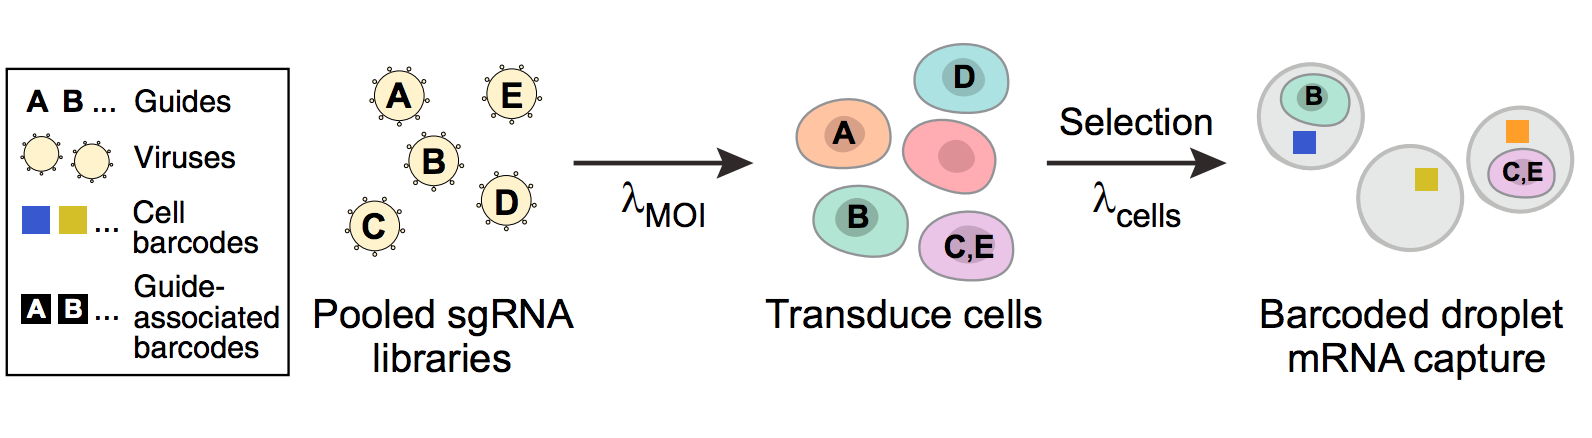
\includegraphics[width=\textwidth]{overview.png}
    \caption{\textbf{A graphical overview of the generalized linear model fit in Perturb-Seq analyses.} \newline \newline
    \label{fig:overview}}
\end{figure}

\section*{Introduction}
In three recent papers published in the journal \textit{Cell}, researchers at the Broad Institute, UCSF, and the Weizmann Institute described a new technology called Perturb-Seq, which integrates CRISPR-Cas9 genome editing and droplet-based single-cell RNA-Seq. \textbf{Figure \ref{fig:overview}} Additionally, a well-crafted Perturb-Seq experiment could enable the dissection gene regulation in the context of disease.


 Basically they use CRISPRi to knockdown different genes in different cells, then examine the transcriptome outcome of the different knockdowns through single-cell RNA-seq. Very often after a genome-wide CRISPR screen, you often have many hits, so they can use CRISPRi to validate each hits and explore the mechanism of the KD effect. Although single-cell readout from Drop-Seq could be noisy, they sequence ~500 cells per CRISPRi, so the average from the ~500 should give a much more robust expression readout. 

\begin{figure}[ht]
    \centering
    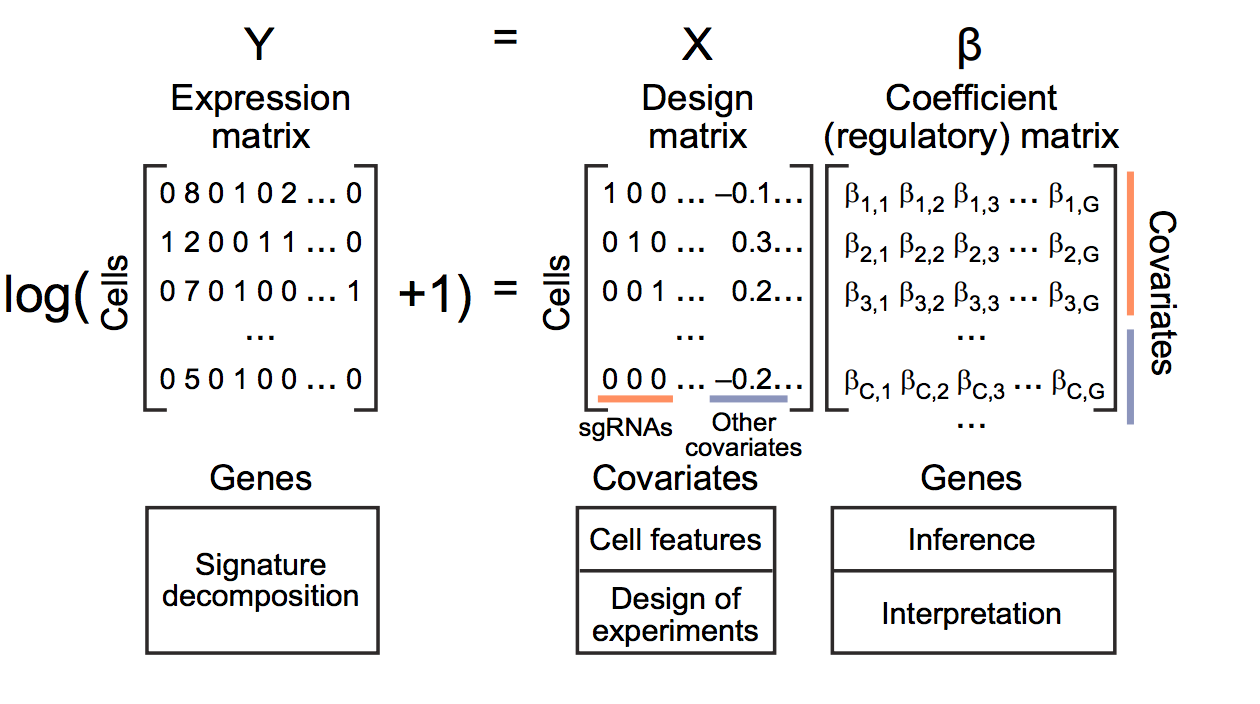
\includegraphics[width=\textwidth]{model.png}
    \caption{\textbf{A graphical overview of the generalized linear model fit in Perturb-Seq analyses.}}
     \label{fig:model}
\end{figure}


\section*{Where the stats are now}

\section*{Links to the BST245 Course}

\section*{Presentation Outline}
\begin{itemize}
  \item 0-6 minutes: discussion of CRISPR, scRNA-Seq, Drop-Seq, and requisite technological innovations as background
  \item 6-10 minutes: introduction of Perturb-Seq
  \item 
\end{itemize}


\section*{References}
Adamson, Britt, et al. "A multiplexed single-cell CRISPR screening platform enables systematic dissection of the unfolded protein response." Cell 167.7 (2016): 1867-1882. \newline \newline
Dixit, Atray, et al. "Perturb-seq: dissecting molecular circuits with scalable single-cell RNA profiling of pooled genetic screens." Cell 167.7 (2016): 1853-1866. \newline \newline
Jaitin, Diego Adhemar, et al. "Dissecting Immune Circuits by Linking CRISPR-Pooled Screens with Single-Cell RNA-Seq." Cell 167.7 (2016): 1883-1896. \newline \newline
Wagner, Daniel E., and Allon M. Klein. "Genetic screening enters the single-cell era." Nature Methods 14.3 (2017): 237-238.
\end{document}
